\chapter{Numerical Methods for Acoustic Inverse Design}\label{sec:methods}

% The aim of this thesis is to use inverse design to find a phononic beamsplitter,
% a task that can be divided into three parts: 
% First, some definitions of what
% should be designed and what constitutes a ``good'' design needs to be made.
% Second, a way to calculating the gradient of the ``goodness'' with respect
% to the design is needed.
% And lastly, we need a gradient based optimization algorithm to find the optimal
% design.
% All of this will be described in this chapter.
The aim of this thesis was to use inverse design to find a phononic
beamsplitter. In this section we describe how that was accomplished. First I
specify the skeleton of the device, i.e.\ the parts that were fixed, as well as
the objective function. We then go on to specify how the simulations and
optimization was done.

\section{Design}

The skeleton of the device to be optimized can be seen in \cref{fig:bs-design}.
The input and output waveguides consist of unit cells like the one in
\cref{fig:unitcell}.
The values for the parameters in the sketch are given in \cref{tab:params}.
The reason for using this mode in this waveguide is that it has been shown to be
interesting for avoiding mechanical leakage into the substrate on which it is
clamped, as well as retaining a high optomechanical
coupling~\cite{kolvik_clamped_2023}.

The design placed in the design area was one of two types.
The first was a \emph{continuous design}, meaning that the material parameters
$\rho$ and $C_{ijkl}$ varied continuously. The range of values that they
can take are between the density and elasticity of pure silicon and that of air.
realized, but was useful as a first step in the optimization.
This was parametrized through the \emph{design field}, $p$, which took values
between 0, pure air, and 1, pure silicon.
The second kind was a binary design, where each point either had silicon or not
with no in-between values.
This was accomplished using level-set methods, which will be explained in
\cref{sec:level-set}.
Because the device was completely symmetric, only one half of it needed to be
modeled, and the other half extrapolated through a symmetry boundary condition.

\begin{figure}[htpb]
	\centering
	\def \a{0.5}
\def \w{1.0}
\def \hx{0.13}
\def \hy{0.3}

\tikzset{
	unitcell/.pic={
		\draw[pic actions] (-0.5*\a, -0.5*\w) rectangle (0.5*\a, 0.5*\w);
		\draw[fill=white] (0, 0) circle [x radius=\hx, y radius=\hy];
	}
}

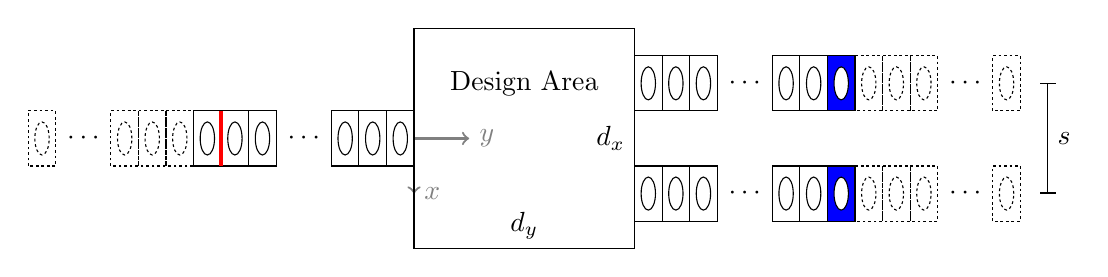
\begin{tikzpicture}[scale=0.7]
	\def \designx{4.0}
	\def \designy{4.0}
	\def \outputh{1.0}
	\def \nunitcells{16}
	\def \nnonpmls{10}

	% Coordinate system
	\draw[gray, thick, ->] (0,0) -- (0,-1) node [anchor=west] {$x$};
	\draw[gray, thick, ->] (0,0) -- (1,0) node [anchor=west] {$y$};

	% Input waveguide
	\path
		(-0.5*\a, 0) pic[transform shape] {unitcell}
		(-1.5*\a, 0) pic[transform shape] {unitcell}
		(-2.5*\a, 0) pic[transform shape] {unitcell}
		(-4.0*\a, 0) node {$\cdots$}
		(-5.5*\a, 0) pic[transform shape] {unitcell}
		(-6.5*\a, 0) pic[transform shape] {unitcell}
		(-7.5*\a, 0) pic[transform shape] {unitcell};
	\draw[red, ultra thick]
		(-7*\a, -0.5*\w) --
		(-7*\a, +0.5*\w);
	\begin{scope}[dash=on 1pt off 1pt phase 0pt]
	\path
		(-8.5*\a, 0) pic[transform shape] {unitcell}
		(-9.5*\a, 0) pic[transform shape] {unitcell}
		(-10.5*\a, 0) pic[transform shape] {unitcell}
		(-12.0*\a, 0) node {$\cdots$}
		(-13.5*\a, 0) pic[transform shape] {unitcell};
	\end{scope}

	% Design area
	\draw (0, -\designx / 2) rectangle (\designy, \designx / 2);
	\node at (\designy / 2, 1) {Design Area};
	\node[left] at (\designy, 0) {$d_x$};
	\node[above] at (\designy/2, -\designx/2) {$d_y$};

	% Output waveguide
	\begin{scope}[xshift=\designy cm, yshift=\outputh cm]
	\path
		(0.5*\a, 0) pic[transform shape] {unitcell}
		(1.5*\a, 0) pic[transform shape] {unitcell}
		(2.5*\a, 0) pic[transform shape] {unitcell}
		(4.0*\a, 0) node {$\cdots$}
		(5.5*\a, 0) pic[transform shape] {unitcell}
		(6.5*\a, 0) pic[transform shape] {unitcell}
		(7.5*\a, 0) pic[transform shape, fill=blue] {unitcell};
	\begin{scope}[dash=on 1pt off 1pt phase 0pt]
	\path
		(8.5*\a, 0) pic[transform shape] {unitcell}
		(9.5*\a, 0) pic[transform shape] {unitcell}
		(10.5*\a, 0) pic[transform shape] {unitcell}
		(12.0*\a, 0) node {$\cdots$}
		(13.5*\a, 0) pic[transform shape] {unitcell};
	\end{scope}
	\end{scope}
	\begin{scope}[xshift=\designy cm, yshift=-\outputh cm]
	\path
		(0.5*\a, 0) pic[transform shape] {unitcell}
		(1.5*\a, 0) pic[transform shape] {unitcell}
		(2.5*\a, 0) pic[transform shape] {unitcell}
		(4.0*\a, 0) node {$\cdots$}
		(5.5*\a, 0) pic[transform shape] {unitcell}
		(6.5*\a, 0) pic[transform shape] {unitcell}
		(7.5*\a, 0) pic[transform shape, fill=blue] {unitcell};
	\begin{scope}[dash=on 1pt off 1pt phase 0pt]
	\path
		(8.5*\a, 0) pic[transform shape] {unitcell}
		(9.5*\a, 0) pic[transform shape] {unitcell}
		(10.5*\a, 0) pic[transform shape] {unitcell}
		(12.0*\a, 0) node {$\cdots$}
		(13.5*\a, 0) pic[transform shape] {unitcell};
	\end{scope}
	\end{scope}
	\draw[|-|]
		(15*\a + \designy, -\outputh) -- node[right] {$s$}
		(15*\a + \designy, \outputh);
		
\end{tikzpicture}

	\caption{
		Device design to be optimized.
		At the red line, a wave traveling right was excited.
		The output was measured over the blue unit cells.
		The dashed unit cells marks \glspl{pml}.
		The large, rectangular design area has dimensions $d_x \times d_y \times
		h$.
	}
	\label{fig:bs-design}
\end{figure}

\begin{table}[htpb]
	\centering
	\caption{%
		Values for the geometric parameters of the device.
		Reference \cref{fig:bs-design,fig:unitcell} for what the quantities
		mean.
	}%
	\label{tab:params}

	\begin{tabular}{cc}
		\toprule
		Parameter & value\\
		\midrule
		$a$ & \qty{187}{\nm}\\
		$w$ & \qty{187}{\nm}\\
		$h_x$ & \qty{153.5}{\nm}\\
		$h_y$ & \qty{49.5}{\nm}\\
		$h$ & \qty{220}{\nm}\\
		$d_x$ & $6 w$\\
		$d_y$ & $4 w$\\
		$s$ & $3 w$\\
		\bottomrule
	\end{tabular}
\end{table}

\subsection{Objective Function}

The figure of merit of the device was the fraction of the input power transmitted
into the output beams.
Furthermore, the power in the output beams was to exit in the same mode as was
excited at the input.
Therefore, a mode overlap integral was used:
\begin{equation}
	I = \int_{\Omega_1} \vec{u}(\vec{x}) \cdot \vec{u}_m^*(\vec{x}) \dl{\vec x},
\end{equation}
where $\vec u_m$ is the shape of the mode (\cref{fig:ms1}).
Because we were not interested in the phase of the output waves,
the absolute value squared of the overlap integral was taken as the objective
function,
\begin{equation}
	\fobj = \abs{I}^2 = I I^*.
\end{equation}
This is maximal when the excitation of the mode $m$ in the output
waveguide is maximized, regardless of which phase it has.
Note that because symmetry is enforced, the power through both outputs will be
the same, and the outgoing waves will have the same phases.

The functional derivative of $\fobj$ with respect to $p$ then becomes
\begin{align}
	\diff.f.{\fobj}{p}(x) &= \diff.f.{I}{p}(x) I^* + I\diff.f.{I^*}{p}(x)\\
	&= \diff.f.{I}{p}(x) I^* + \left(I^*\diff.f.{I}{p}(x)\right)^*\\
	&= 2\Re\left(\diff.f.{I}{p}(x) I^*\right).
\end{align}
The derivative of $I$ was derived in \cref{sec:spec_der}.

\subsection{Excitation}\label{sec:excitation_method}

\tododec{JK thinks a figure or more is apt here?}
\tododec{%
	\emph{%
		RVL: As we discussed once, I feel you actually need more than one
		boundary to excite exactly one mode, or you don't have wavevector
		information on the incoming mode? I presume this is why you get a backward
		propagation mode at excitation point? Please add some explanation.
	}
	\\
	We don't need (and shouldn't have I think) more boundaries. The wavevector
	information is partly given through frequency and partly through the profile
	of the force added. The reason for the backward propagating mode is that the
	boundary stress would be the same for a backward traveling wave. One could
	add a force on the next boundary over to cancel the backward
	propagating wave from the first boundary load, but then that would create
	another backward propagating wave. Perhaps this would be of smaller
	magnitude
}

To excite the input waveguide in the desired mode,
the stress on the boundary of a unit cell was exported from a unit cell
eigenmode simulation with $k=0.9 \pi / a$ and applied to the boundary marked in red in
\cref{fig:bs-design}.
Since the frequency was perfectly controlled, this excites only the desired
mode, since that is the only permitted mode close by as seen in the band diagram
in \cref{fig:banddiagram}.

In order to confirm that the excitation was indeed fully in the desired mode, a
separate model with only a waveguide with 200 unit cells was created.
After applying the excitation and running the simulation,
the proportion of the excitation that ended up in the desired mode was
calculated.
This was done by first calculating the mode overlap integral
$\int \vec u \vec u_m^* \dl{\vec x}$
and comparing that to the norm of the displacement field
$\int \vec u \vec u^* \dl{\vec x}$.
If $\vec u$ is written as $\vec u = a \vec u_m + b \vec u_r$ where $a$ and $b$
are scalars and $\vec u_r$ is orthogonal to $\vec u_m$,
then
$\int \vec u \vec u^* \dl{\vec x} = a\int \vec u \vec u_m^*\dl{\vec x} + b\int
\vec u \vec u_r^*\dl{\vec x}$.
And since $\vec u_r$ is orthogonal to $\vec u_m$,
$a = \int \vec u \vec u_m^*\dl{\vec x} / \int \vec u_m \vec u_m^*\dl{\vec x}$,
which enables us to calculate $b$ as well.
The result was near perfect ($b < 0.03 a$) excitation of only the desired mode.
Since energy is proportional to
the square of the amplitude, $b < 0.03 a$ means that $>99.9 \%$ of the energy was
in the correct mode.
To obtain such high fidelity, it was important that the mesh used for the
unit cells in the wave guide was the same as the mesh in the unit cell
simulation.
High fidelity was also achieved if both meshes were made very fine, but such
fine meshes carries a prohibitively large computational cost.

\subsection{Perfectly Matched Layers (PMLs)}

Ideally, the input and outputs are infinite waveguides.
Unfortunately, infinitely large models require infinite simulation time, which
is problematic.
Instead, \glspl{pml} were placed at the caps of the input and output waveguides.
The purpose of the \gls{pml} was to absorb any incoming waves without reflection,
which would make it act as if there was an infinite waveguide on the other side
into which the waves propagate indefinitely.
One way to accomplish this is to add an imaginary component to the density of
the material.
\todowrt{why does it work}
The imaginary part must be introduced smoothly,
otherwise the abrupt change in material
parameters would induce reflections anyway.
Therefore, the imaginary part was taken to be exponentially increasing,
\begin{equation}\label{eq:rho_im}
	\rho_\text{im} = \rho_\text{si} \cdot s \cdot
	\frac{e^{-\abs{y-y_0} / d} - e^{-n/d}}{1 - e^{-n/d}}.
\end{equation}
In this equation, $y_0$ is the point where the waveguide ends,
$n$ is the length of the \gls{pml}, $d$ decides the steepness of the
exponential and $s$ the final value.
\Cref{fig:pml_profile} shows the effect of changing these parameters on the
shape of the profile of the imaginary component.

\begin{figure}[htpb]
	\centering
	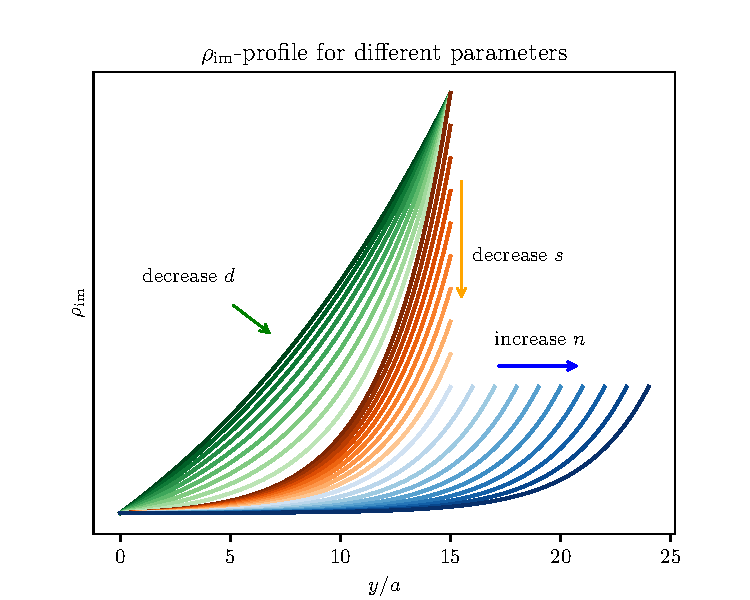
\includegraphics{chapters/methods/pml_profile.pdf}
	\caption{%
		This figure shows the effect of changing the different parameters in
		\cref{eq:rho_im}.
		The green curves shows changing $d$ while keeping the other parameters
		fixed, and the orange and blue show $s$ and $n$ respectively.
		Darker colour means higher value, and the last green curve coincides
		with the first orange, and the last orange with the first blue.
	}%
	\label{fig:pml_profile}
\end{figure}

There are three possible sources of reflections from the \gls{pml} region.
Firstly, if the transition from no imaginary component to some imaginary
component is too abrupt, that causes reflections.
Secondly, if the imaginary component is too small, the waves will not be
completely dampened when they reach the end of the \gls{pml} and thus reflect
off of that.
And lastly, if $d$ is small then there can be reflections from the steep
increase that happens some distance away from the beginning of the \gls{pml}.
See \cref{fig:banddiagram} for an illustration of where the different types of
reflections occur.

\tikzset{
	reflection/.pic={
		\draw[->] (-0.4, 0) -- (-0.1, 0) arc[radius=0.1, start angle=-90, end
		angle=90] --++ (-0.1, 0);
		\draw[dashed] (0,-3.1) -- (0,8.3);
	}
}
\begin{figure}[htpb]
	\centering
	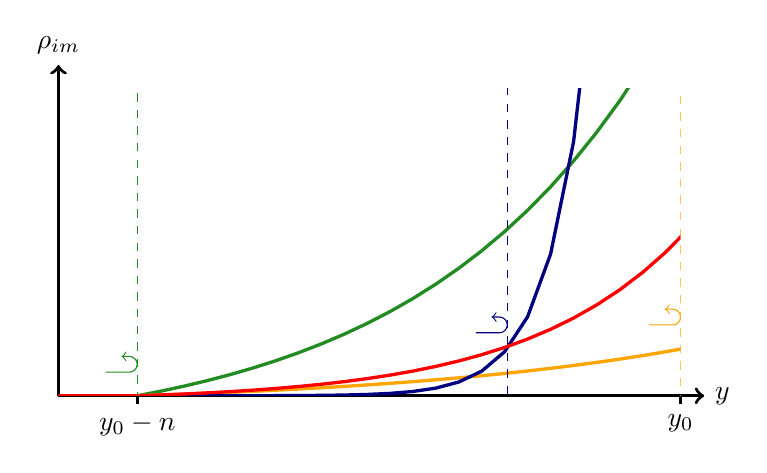
\begin{tikzpicture}[domain=1:8]

		\draw[->,very thick] (-0.0,0) -- (8.2,0) node[right] {$y$};
		\draw[->,very thick] (0,-0.0) -- (0,4.2) node[above] {$\rho_\text{im}$};
		\draw[very thick] (1,0) -- (1,-0.10) node[below] {$y_0-n$};
		\draw[very thick] (7.9,0) -- (7.9,-0.10) node[below] {$y_0$};
		%\draw[very thin,color=gray] (-0.1,-1.1) grid (7.9,3.9);
		\clip (0.0, 0.0) rectangle (7.9,3.9);
		\draw[color=ForestGreen, very thick] (0,0) -- (1,0) --
			plot (\x,{0.40*(exp(\x/3)-exp(1/3))});
		\draw[color=Orange, very thick] (0,0) -- (1,0) --
			plot (\x,{0.10*(exp(\x/4)-exp(1/4))});
		\draw[color=NavyBlue, very thick] (0,0) -- (1,0) --
			plot (\x,{0.02*exp(2.0*(\x-4))});
		\draw[color=Red, very thick] (0,0) -- (1,0) --
			plot (\x,{0.04*(exp(\x/2)-exp(1/2))});
		\draw[ForestGreen] (1.0, 0.3) pic {reflection};
		\draw[NavyBlue] (5.7, 0.8) pic {reflection};
		\draw[Orange] (7.9, 0.9) pic {reflection};
	\end{tikzpicture}
	\caption{%
		For the green curve, the initial sudden increase of the imaginary
		component of the density at the beginning of the \gls{pml} causes reflections.
		For the blue curve, the beginning of the \gls{pml} is smooth but there
		is an increase partway through sharp enough to cause reflections.
		For the orange curve, the \gls{pml} never becomes strong enough to
		completely dampen the waves, and they get reflected at the end.
		The red curve balances all these, yielding a perfect, reflectionless
		\gls{pml}.
	}%
	\label{fig:pml_reflections}
\end{figure}

It was desirable to make $n$ as small as possible while still eliminating all
reflections.
This was because a smaller $n$ meant a smaller model which resulted in shorter
simulation times.
In order to do so, a long waveguide with the same parameters as
used for the input and output waveguides in the beamsplitter design was created.
To discern where there was some component of the wave reflected, a fourier
transform of the displacement field was made.
The parameters controlling the shape of the $\rho_\text{im}$ curve were then
varied and an appropriate value was selected.

\subsection{Level-Set}\label{sec:level-set}

Ultimately, we wanted the device to consist of regions of material and regions of
no material.
Such a design is defined by the boundary between filled and empty regions.
How to best implement a method of storing and evolving this boundary requires
some thought.
The first, and perhaps most intuitive implementation,
would be to simply store the coordinates of evenly spaced points on the boundary.
In addition to storing the coordinates, one must also store which points
neighbour which.
A different method, which is the one used in this report, is called
the \emph{level-set method}.
With this method, the boundary is not directly stored, but is rather stored via an
\emph{implicit function}, $\phi(x)$,
and the boundary is recovered as the
0-isocontour of $\phi$, i.e.\ the points $x$ where $\phi(x)=0$.

There are two main advantages of using the level-set method rather than
directly storing the boundary points.
Firstly, when moving the boundary we would like to do so in the normal
direction, as moving it along itself has no effect.
Computing the normal direction of a directly stored boundary is slightly cumbersome,
though certainly achievable.
With level-set, moving the boundary in the normal direction is as easy as adding
a constant to the implicit function.
Secondly, while the boundary is changing, the resolution in one part might need
to be increased while the resolution in another needs to be decreased. Deciding
where and when to add new points is non-trivial when directly storing the
boundary. Furthermore, if two domains merge, or if one splits, points
need to be removed and the connectivities changed, which is difficult.
\Cref{fig:direct_troubles} illustrates these problems with direct storage concretely.
Both of these issues are automatically handled with the level-set method, as
shown in \cref{fig:signed_dist_example}.

\begin{figure}[htpb]
	\centering
	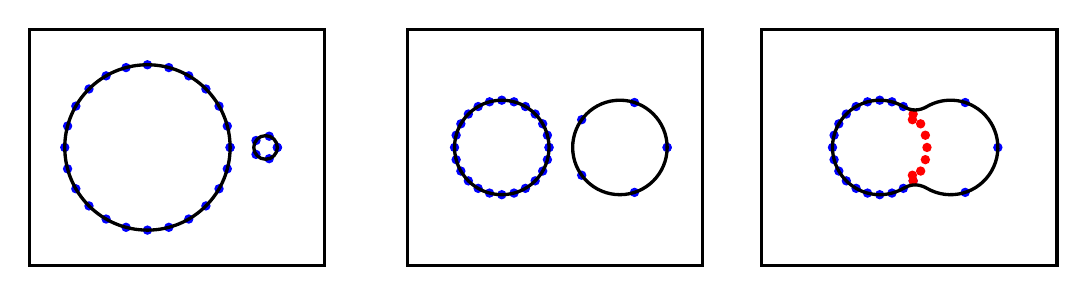
\begin{tikzpicture}[scale=1.5, very thick]
	\coordinate (ca) at (0,0);
	\coordinate (cb) at (1,0);
	\def\radiusa{0.7cm}
	\def\radiusb{0.1cm}
	\def\radpt{0.7pt}
	\draw (-1,-1) rectangle (1.5,1);
	\foreach \i in {0,15,...,360}{% 
		\filldraw [blue]  (ca)++(\i:\radiusa) circle (\radpt);
	}
	\foreach \i in {0,72,...,360}{% 
		\filldraw [blue]  (cb)++(\i:\radiusb) circle (\radpt);
	}
	\draw (ca) circle[radius=\radiusa];
	\draw (cb) circle[radius=\radiusb];

	\begin{scope}[xshift=3cm]
		\coordinate (ca) at (0,0);
		\coordinate (cb) at (1,0);
		\def\radiusa{0.4cm}
		\def\radiusb{0.4cm}
		\draw (-0.8,-1) rectangle (1.7,1);
		\foreach \i in {0,15,...,360}{% 
			\filldraw [blue]  (ca)++(\i:\radiusa) circle (\radpt);
		}
		\foreach \i in {0,72,...,360}{% 
			\filldraw [blue]  (cb)++(\i:\radiusb) circle (\radpt);
		}
		\draw (ca) circle[radius=\radiusa];
		\draw (cb) circle[radius=\radiusb];
	\end{scope}
	\begin{scope}[xshift=6cm]
		\coordinate (ca) at (0.2,0);
		\coordinate (cb) at (0.8,0);
		\def\radiusa{0.4cm}
		\def\radiusb{0.4cm}
		\draw (-0.8,-1) rectangle (1.7,1);
		\foreach \i in {60,75,...,315}{% 
			\filldraw [blue]  (ca)++(\i:\radiusa) circle (\radpt);
		}
		\foreach \i in {-72,0,72}{% 
			\filldraw [blue]  (cb)++(\i:\radiusb) circle (\radpt);
		}
		\foreach \i in {-45, -30, ..., 45}{% 
			\filldraw [red]  (ca)++(\i:\radiusa) circle (\radpt);
		}
		\foreach \i in {144, -144}{% 
			\filldraw [red]  (cb)++(\i:\radiusb) circle (\radpt);
		}
		\draw (ca)++(60:\radiusa)
			arc[radius=\radiusa, start angle=60, end angle=300]
			to[out=30, in=150]
			([shift=(240:\radiusb)] cb)
			arc[radius=\radiusb, start angle=240, end angle=480]
			to[out=210, in=-30]
			cycle;
		%\draw (cb) circle[radius=\radiusb];
	\end{scope}
\end{tikzpicture}

	\caption{%
		Possible evolution of boundary. In the leftmost figure, the
		boundary is defined by pretty much evenly spaced points. In the center figure
		the boundaries have moved and the spacing is no longer even, and the
		right circle is very poorly resolved.
		The rightmost figure shows the boundary after the two circles moved
		closer together. Now there are multiple points that need to be removed,
		marked in red, and the connectivity of the points that remain must be
		changed such that the two boundaries are merged.
	}%
	\label{fig:direct_troubles}
\end{figure}
\begin{figure}[htpb]
	\centering
	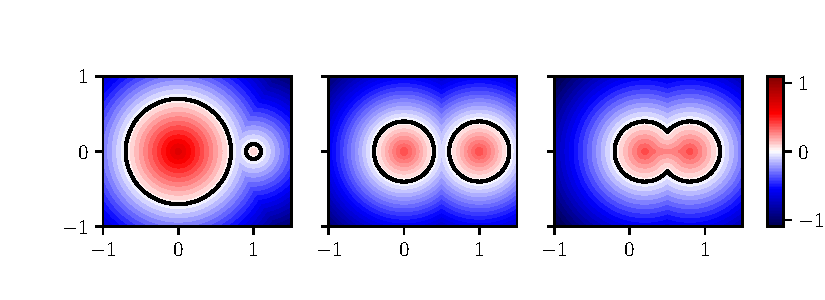
\includegraphics{chapters/methods/signed_dist_example.pdf}
	\caption{%
		Signed distance function for the boundaries in
		\cref{fig:direct_troubles}. The resolution of the boundary depends only
		on the resolution of the signed distance field, and not on how the
		boundary moves, so evolving boundaries will never become poorly
		resolved. Additionally,
		topological changes are also smoothly handled since there is no need to
		explicitly specify connectivities.
	}%
	\label{fig:signed_dist_example}
\end{figure}

There are of course a lot of possible functions $\phi(x)$ that have a given
boundary as it's 0-isocontour.
There is one choice that simplifies a lot of calculations though: the signed
distance function.
This function is defined as the distance from the closest point on the boundary,
with a plus sign if it is inside and a minus sign if it is outside the boundary.
See \cref{fig:signed_dist_example} for an example.
It has the advantage that if one wishes to locally shift the boundary some
length $s$ in the normal direction, then simply add $s$ to the function there.
\Cref{fig:add_shift} shows this effect in one dimension.
\todowrt{%
	Create another figure that shows it in two dimensions.
	I'm thinking a circular boundary, and adding $s$ in the left half and
	subtracting $s$ in the right half. Alternatively adding $s\cdot x$ (unit circle
	centered on 0) so that it will be smooth
}

\begin{figure}[htpb]
	\centering
	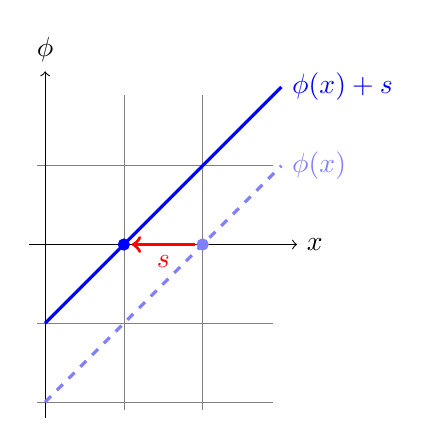
\begin{tikzpicture}[domain=0:3]
		\draw[very thin,color=gray] (-0.1,-2.1) grid (2.9,1.9);

		\draw[->] (-0.2,0) -- (3.2,0) node[right] {$x$};
		\draw[->] (0,-2.2) -- (0,2.2) node[above] {$\phi$};
		\draw[color=blue!50, dashed, very thick] plot (\x,{\x-2})
			node[right] {$\phi(x)$};
		\draw[color=blue, very thick] plot (\x,{\x-1})
			node[right] {$\phi(x)+s$};
		\filldraw[color=blue!50] (2,0) circle[radius=2pt];
		\filldraw[color=blue]    (1,0) circle[radius=2pt];
		\draw[color=red, ->, very thick] (1.9,0) --
			node[below] {$s$}
			(1.1,0);
	\end{tikzpicture}
	\caption{Adding $s$ to the signed distance function shifts boundary by
	$s$.}%
	\label{fig:add_shift}
\end{figure}

Using a signed distance function means that a gradient descent step could be taken
by simply adding the gradient field to the signed distance field.
However, there are some pitfalls that had to be avoided.
Firstly, the gradient needed to be rescaled so that the boundary moved
an appropriate distance.
This was done such that the boundary moves at most \qty{1}{\nm}.
\todoblk[noinline]{check this number before finalizing, we change it every now and then}
Secondly, since the gradient was occasionally sharply peaked somewhere
far from the boundary, only the gradient near the boundary is actually added
to the signed distance field.
After performing this addition, what was previously a signed distance field
would now no longer be that, and thus the signed distance field was recalculated from
the new, shifted boundary.
This recalculation came with a performance penalty, but since the COMSOL
simulations were orders of magnitude slower than all other parts of the
optimization, this was of little concern.


\section{Optimization}\label{sec:m_optimization}

For the optimization, we used the \gls{adam}
algorithm with one modification:
a global learning rate was employed rather than
separate learning rates for each dimension.
The reasoning for this was that separate learning
rates would give jagged contours, which might not be properly resolved by the
meshing. Practically this modification means that \mintinline{Python}+v+ is a
scalar and is set to \mintinline{Python}{(1-beta_2)*np.mean(g**2) + beta_2 * v}
in \cref{lst:adam}.
The optimization was run and continually monitored, and once convergence was
visually confirmed through looking at the plot of $\fobj$ by iteration, it was terminated.
A few different values for the $\beta$:s were tried, and in the end
$\beta_1=0.9$ and $\beta_2 = 0.95$ were chosen.
However, it seemed that the evolution were not too sensitive to this choice.
$\alpha$ was taken to be \num{2e-3}, because that is large enough that $p$
could change from 0 to 1 in 500 iterations, which was deemed an appropriate
timescale as the time per iteration was about 4 minutes.
A too large $\alpha$ would lead to poor convergence, while a too low value would
result in slow progress.

The final step of the optimization was to use level-set for the design.
However, just using the $p=0.5$ boundary of the final optimized continuous
design as the initial point of the level-set optimization would be an abrupt
change, and there is no reason to expect that the resulting level-set design
would be close to a design with good performance.
Therefore, once the continuous optimization had converged, a sigmoid function
was applied to the design field $p$ before $\rho$ and $C_{ijkl}$ were set:
\begin{align}
	\rho(\vec x) &= \rho_\text{si} \sigma_r(p(\vec x)),
	&
	C_{ijkl}(\vec x) &= C_{ijkl}^\text{si} \sigma_r(p(\vec x)),
	&
	\sigma_r(p) = \frac{1}{1+e^{-(p-0.5)/r}}.
\end{align}
and then the optimization was restarted.
The sigmoid results in fewer values close to 0.5, effectively making the device
closer to being binary, which means that the step to level-set designs wasn't as
abrupt.
Note that the parameter $r$ controls how much values are shifted, and with
$r\to 0$, $\sigma_r$ becomes a step function.
Once that had been repeated a couple of times with decreasing $r$,
the level-set design was
initialized using the $p=0.5$ boundary of the final optimized design,
and the level-set optimization was run.

\section{Simulations}

In this section we detail some of the practicalities of performing the
simulations.
For finite element simulations we used COMSOL version 6.0.
First, a unit cell with periodic boundary conditions was simulated,
from which we obtained:
\begin{itemize}
	\item the mode shape, used to calculate the component of the displacement
		field in the desired mode,
	\item the stress at the boundary, used as the force exciting the input
		waveguide,
	\item the frequency at which to excite in order to obtain a traveling wave
		with the desired wave vector.
	\item a mesh to be used when meshing the unit cells in the waveguides.
\end{itemize}

For the continuous optimization, the basic procedure went
\begin{enumerate}
	\item Through the COMSOL-Matlab API, a beamsplitter model was made.
		The excitation force profile as well as the unit cell mesh and the mode
		shape were imported from the unit cell simulation.
	\item A semi-random initial design field $p$ was created. This was done by
		drawing a sample from a Gaussian process, which means that the characteristic
		length scale that the design varies on could be controlled.
	\item\label{it:sigmoid} If the sigmoid function was to be used in this optimization, it was
		applied to the design field, and the result was saved to a different
		variable, that we call the interpolation field.
	\item The interpolation field was imported to the COMSOL model, and the
		material parameters adjusted proportional to said field.
	\item Both forward and backward simulations were run and the gradient was
		calculated and exported to Matlab.
	\item With the gradient, the design field was updated and the algorithm
		returned to step~\ref{it:sigmoid}.
\end{enumerate}

For the level-set optimization, the procedure was basically the same, with some
minor differences:
\begin{enumerate}
	\item Through the COMSOL-Matlab API, a beamsplitter model was made.
		The excitation force profile as well as the unit cell mesh and the mode
		shape was imported from the unit cell simulation.
	\item An initial signed distance field $s$ was created.
		This was done by finding the $p=0.5$ isocontour from the final iteration
		of the continuous optimization, and initializing a signed distance field
		from that.
	\item\label{it:import} The zero isocontour of the signed distance field was imported into
		the COMSOL model and a geometry was built from that.
	\item Both forward and backward simulations were run and the gradient was
		calculated and exported to Matlab.
	\item With the gradient, the signed distance field was updated and the algorithm
		returns to step~\ref{it:import}.
		Note that as part of the update, the signed distance field was
		reinitialized so that it would not lose its properties.
\end{enumerate}
